\begin{center}
\Huge
Cirklens ligning
\end{center}

\section*{Cirklens ligning}
\stepcounter{section}
Præcist som det er tilfældet for linjen kan vi bestemme en ligning for en cirkel. 
\begin{setn}[Cirklens ligning]
	Cirklen $C$ med centrum i $(x_0,y_0)$ og radius $r$ har ligningen
	\begin{align*}
		(x-x_0)^2 + (y-y_0)^2 = r^2.
	\end{align*}
\end{setn}
\begin{proof}
	Lad $(x,y)$ være et punkt på cirklen $C$, og lad $(x_0,y_0)$ være cirklens centrum. Så er
	forbindelsesvektoren $\vv{v}$ mellem $(x,y)$ og $(x_0,y_0)$ givet ved
	\begin{align*}
		\vv{v} = 
		\begin{pmatrix}
			x-x_0 \\
			y-y_0
		\end{pmatrix}.
	\end{align*}
	Da radius for $C$ er $r$, så skal længden af $\vv{v}$ være $r$. Dette medfører
	\begin{align*}
		r = |\vv{v}| = \sqrt{(x-x_0)^2+(y-y_0)^2}. 
	\end{align*}
	Vi opløfter nu begge sider af lighedstegnet i anden og får
	\begin{align*}
		r^2 = \left(\sqrt{(x-x_0)^2+(y-y_0)^2}\right)^2 = (x-x_0)^2 + (y-y_0)^2.
	\end{align*}
\end{proof}

\begin{figure}[H]
	\centering
	\begin{tikzpicture}
		\begin{axis}[
			axis lines = middle, 
			xmin = -2, xmax = 8,
			ymin = -2, ymax = 8,
			x = 1cm, y = 1cm,
			ticks = none, 
			xlabel = $x$, ylabel = $y$,
			]
			\draw[-{Stealth[scale = 1.5]},thick, color = olive] (axis cs: 4,4) -- (axis cs: 6.58,5.53);
			\filldraw[color = teal] (axis cs: 4,4) circle (2pt);
			\filldraw[color = teal] (axis cs: 6.58,5.53) circle (2pt);
			\node[color = teal] at (axis cs: 4,3.5) {$(x_0,y_0)$};
			\node[color = teal] at (axis cs: 7,6) {$(x,y)$};
			\draw[decorate,decoration={brace,amplitude=5pt,raise=0.9ex}, color = olive, thick] (axis cs: 4,4) 
			-- (axis cs: 6.58,5.53) node[midway, color = olive, xshift = -1.8ex, yshift = 2.5ex] {$r$};
			\draw[color = teal, thick] (axis cs: 4,4)	 circle (3cm);	
		\end{axis}
	\end{tikzpicture}
	\caption{Cirkel med centrum i $(x_0,y_0)$ og radius $r$.}
\end{figure}

\begin{exa}
	En cirkel har centrum i $(3,2)$ og radius $2$. Cirklens ligning er så
	\begin{align*}
		(x-3)^2 + (y-2)^2 = 4.
	\end{align*}
\end{exa}

\begin{exa}
	En cirkel har ligningen 
	\begin{align}\label{eq:1}
		(x-1)^2 + (y-4)^2 = 16. 
	\end{align}
	Vi skal afgøre, om punktet $(5,4)$ ligger på cirklen. Vi indsætter derfor dette
	i \eqref{eq:1} og får
	\begin{align*}
		(5-1)^2 + (4-4)^2 = 4^2=16,
	\end{align*}
	og da denne lighed er korrekt, så er punktet på cirklen. 
\end{exa}

\section*{Kvadratkomplettering}
\stepcounter{section}

En cirkel med centrum i $(x_0,y_0)$ og radius $r$ har ligningen
\begin{align}\label{eq:1}
	(x-x_0)^2 + (y-y_0)^2 = r^2.
\end{align}
Hæver vi parenteserne i denne ligning, så får vi
\begin{align}\label{eq:2}
	x^2+x_0^2-2xx_0 + y^2+y_0^2-2yy_0 = r^2,
\end{align}
og cirklens ligning vil ofte optræde på denne form. Kvadratkomplettering går ud på at få en ligning fra formen \eqref{eq:2} tilbage på formen \eqref{eq:1}, så radius og centrum kan aflæses.

\begin{exa}
	En cirkel har ligningen 
	\begin{align*}
		x^2-2x+y^2-4y=4.
	\end{align*}
	Vi ser, at vi har leddene $x^2$ og $-2xx_0 = -2x$ samt $y^2$ og $-2yy_0=-4y$. Derfor kan vi se, at $x_0 = 1$ og $y_0 = 2$. Ifølge \eqref{eq:2} skal vi have $x_0^2$
    og $y_0^2$ på venstresiden af lignhedstegnet, så det lægges til i cirklens ligning:
    \begin{align*}
    		x^2-2x+y^2-4y+1+4=4+1+4=9. 
    \end{align*}
   	Da ligningen nu er på formen \eqref{eq:2}, så kan vi se, at cirklen har centrum i $(1,2)$ og radius $\sqrt{9} = 3$.
\end{exa}

\subsection*{Opgave 1}

\begin{enumerate}[label=\roman*)]
	\item Bestem cirklens ligning for cirklen, der har centrum i $(1,2)$
	 og radius $r = 1$.
	\item Bestem cirklens ligning for cirklen, der har centrum i $(0,0)$
	og radius $r = 1$.
	\item Bestem cirklens ligning for cirklen, der har centrum i $(-4,2)$
	og radius $r = 3$.
	\item Bestem cirklens ligning for cirklen, der har centrum i $(\sqrt{2},-\sqrt{3})$
	og radius $r = \sqrt{5}$.
	\item Bestem cirklens ligning for cirklen, der har centrum i $(\frac{1}{3},-\frac{2}{7})$
	og radius $r = \frac{2}{3}$.
\end{enumerate}

\subsection*{Opgave 2}

\begin{enumerate}[label=\roman*)]
	\item Bestem centrum og radius for cirklen med ligningen
	\begin{align*}
		x^2 - 4 x + y^2 - 6 y= -9.
	\end{align*}
	\item Bestem centrum og radius for cirklen med ligningen
	\begin{align*}
		x^2 + 2 x + y^2 + 6 y = -1.
	\end{align*}
	\item Bestem centrum og radius for cirklen med ligningen
	\begin{align*}
		x^2 - 8 x + y^2 + 2 y  = 8.
	\end{align*}
	\item Bestem centrum og radius for cirklen med ligningen
	\begin{align*}
		x^2 - 10 x + y^2 - 12 y  = 3.
	\end{align*}
	\item Bestem centrum og radius for cirklen med ligningen
	\begin{align*}
		x^2 + 4 x + y^2 + 14 y = 47.
	\end{align*}
	
\end{enumerate}

\subsection*{Opgave 3}

\begin{enumerate}[label=\roman*)]
	\item Afgør, om punktet $(1,1)$ ligger på cirklen med ligningen
	\begin{align*}
		(x-1)^2 +(y-2)^2 = 1 
	\end{align*}
	\item Afgør, om punktet $(2,4)$ ligger på cirklen med ligningen
	\begin{align*}
		(x+1)^2 + (y-5)^2 = 49
	\end{align*}
	\item Afgør, om punktet $(1,6)$ ligger på cirklen med ligningen 
	\begin{align*}
		x^2-2x+y^2-4y=11
	\end{align*}
	\item Afgør, om punktet $(-2,2)$ ligger på cirklen med ligningen
	\begin{align*}
		x^2+8x+y^2-8y=32
	\end{align*}
\end{enumerate}

\subsection*{Opgave 4}
Bestem cirklens ligning for følgende cirkler og omskriv dem til formen \eqref{eq:2}.
\begin{center}
	\resizebox{0.45\textwidth}{0.45\textwidth}{
		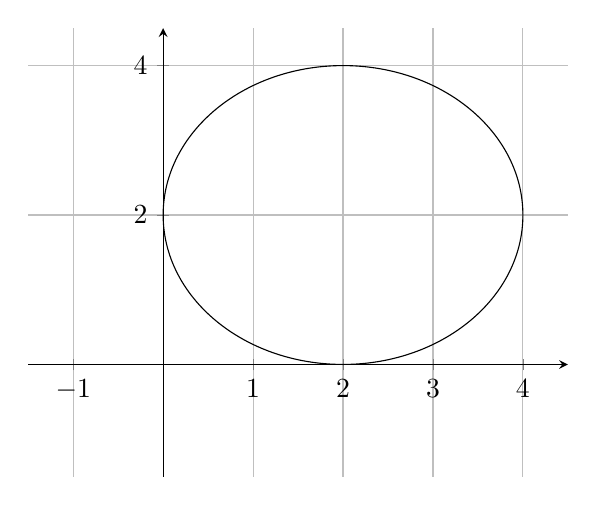
\begin{tikzpicture}
			\begin{axis}[axis lines = middle,
			xmin = -1.5, xmax = 4.5,
			ymin = -1.5, ymax = 4.5, grid]
				\draw (axis cs: 2,2) circle [blue!40, radius = 2];
			\end{axis}
		\end{tikzpicture}
	}
	\resizebox{0.45\textwidth}{0.45\textwidth}{
		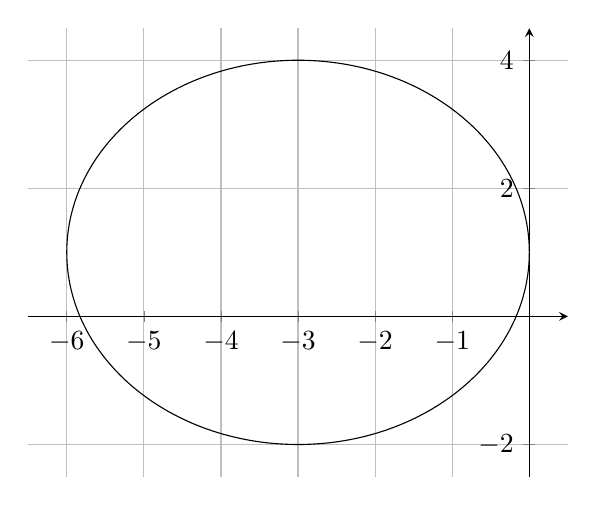
\begin{tikzpicture}
			\begin{axis}[axis lines = middle,
			xmin = -6.5, xmax = 0.5,
			ymin = -2.5, ymax = 4.5, grid]
				\draw (axis cs: -3,1) circle [blue!40, radius = 3];
			\end{axis}
		\end{tikzpicture}
	}
	\resizebox{0.45\textwidth}{0.45\textwidth}{
		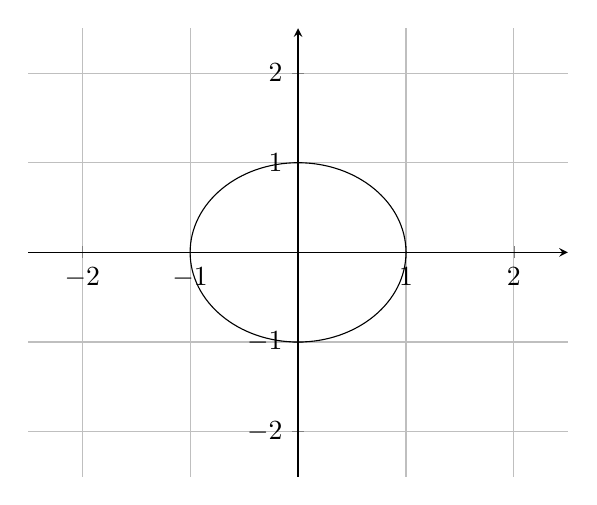
\begin{tikzpicture}
			\begin{axis}[axis lines = middle,
			xmin = -2.5, xmax = 2.5,
			ymin = -2.5, ymax = 2.5, grid]
				\draw (axis cs: 0,0) circle [blue!40, radius = 1];
			\end{axis}
		\end{tikzpicture}
	}
	\resizebox{0.45\textwidth}{0.45\textwidth}{
		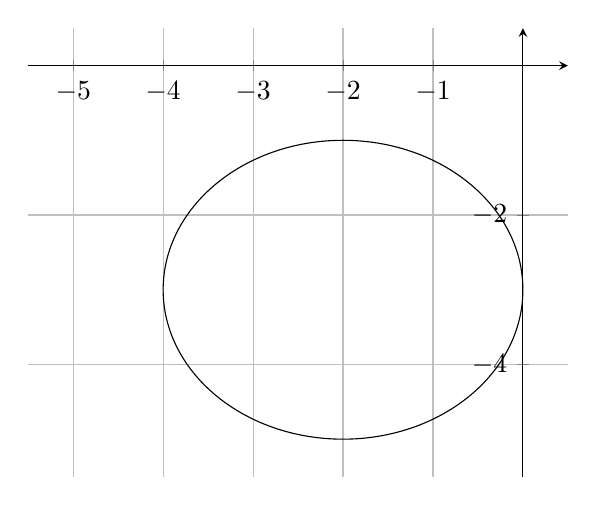
\begin{tikzpicture}
			\begin{axis}[axis lines = middle,
			xmin = -5.5, xmax = 0.5,
			ymin = -5.5, ymax = 0.5, grid]
				\draw (axis cs: -2,-3) circle [blue!40, radius = 2];
			\end{axis}
		\end{tikzpicture}
	}
\end{center}



\subsection*{Opgave 5}
\begin{enumerate}[label=\roman*)]
	\item En cirkel $C$ har centrum i $(-2,-3)$ og radius $r=4$. Afgør, om punktet $(-2,-2)$ 
	ligger på $C$.
	\item En cirkel $C$ har centrum i $(-5,4)$ og radius $r=6$. Afgør, om punktet $(-5,10)$ 
	ligger på $C$.
\end{enumerate}

\subsection*{Opgave 6}
\begin{enumerate}[label=\roman*)]
	\item En cirkel $C$ er givet ved ligningen
	\begin{align*}
		(x+1)^2+(y-t)^2 = 4.
	\end{align*}
	Bestem $t$, så punktet $(1,2)$ ligger på $C$.
	\item En cirkel $C$ er givet ved ligningen
	\begin{align*}
		(x-4)^2 + (y-4)^2 = r^2.
	\end{align*}
	Bestem $r$, så punktet $(4,8)$ ligger på $C$.
	\item En cirkel $C$ er givet ved ligningen
	\begin{align*}
		x^2-10x+y^2-2y=-1.
	\end{align*}
	Bestem $k$, så punktet $(k,1)$ ligger på $C$.
\end{enumerate}




\subsection*{Opgave 7}

\begin{enumerate}[label=\roman*)]
	\item Bestem centrum og radius for cirklen med ligningen
	\begin{align*}
		(x-4)^2+y^2-6y = 27.
	\end{align*}
	\item Bestem centrum og radius for cirklen med ligningen
	\begin{align*}
		x^2+4x+(y-3)^2 = 21.
	\end{align*}
	\item Bestem centrum og radius for cirklen med ligningen
	\begin{align*}
		x^2-14x+(y+5)^2 = 0.
	\end{align*}
\end{enumerate}